%More details on electron reconstruction can be found in Ref.~\cite{ElectronLegacy}. 

Preselection of the electron candidates is made through loose cuts on track-cluster matching observables. This done to maintain highest possible selection efficiency of electrons and to reject QCD background significantly. For the analysis, electrons are subjected to have $p^e_T >$ 7 GeV within $|\eta^e| <$ 2.5, and satisfy a loose primary vertex 
constraints on longitudinal and transvers components of impact parameter $viz.$ $d_{xy} < 0.5$ cm and $d_z < 1$ cm respectively.
Such electrons are called {\bf loose electrons}. Details of electron reconstruction can be explored in Ref.~\cite{ElectronLegacy}.

The data-MC discrepancy is corrected using scale factors as is done for the electron selection with data efficiencies measured through the same tag-and-probe technique outlined later (see Section \ref{sec:eleEffMeas}). 
These studies for reconstructions are carried out by the EGM POG and the results are only summarised here.

The electron reconstruction scale factors are shown Fig. \ref{fig:ele_rec_scale_factors} and are applied as a function of electron $\pt$ and super cluster $\eta$.

\begin{figure}[!htb]
\vspace*{0.3cm}
\begin{center}
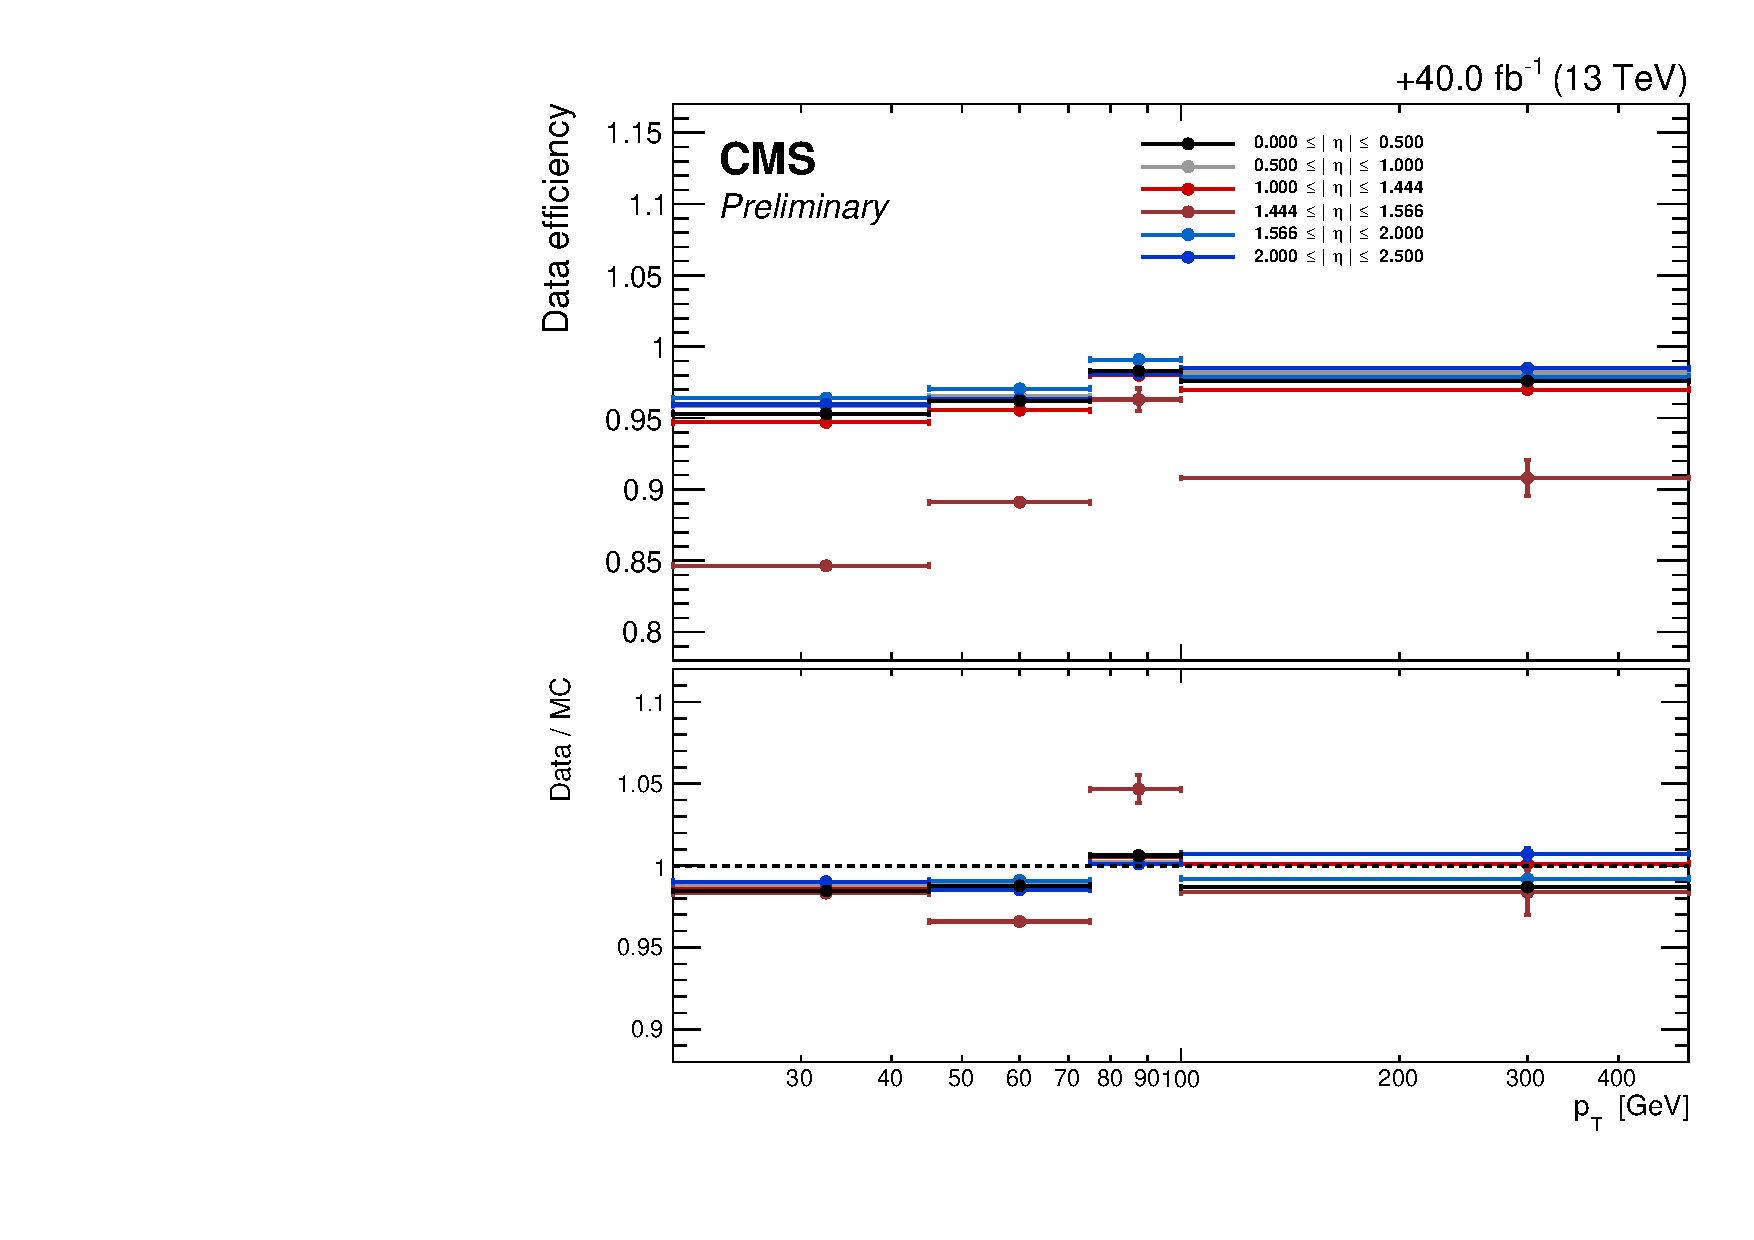
\includegraphics[width=0.4\textwidth]{Figures/Electrons/ErecoPt}
\includegraphics[page=2, width=0.4\textwidth]{Figures/Electrons/ErecoEta}\\
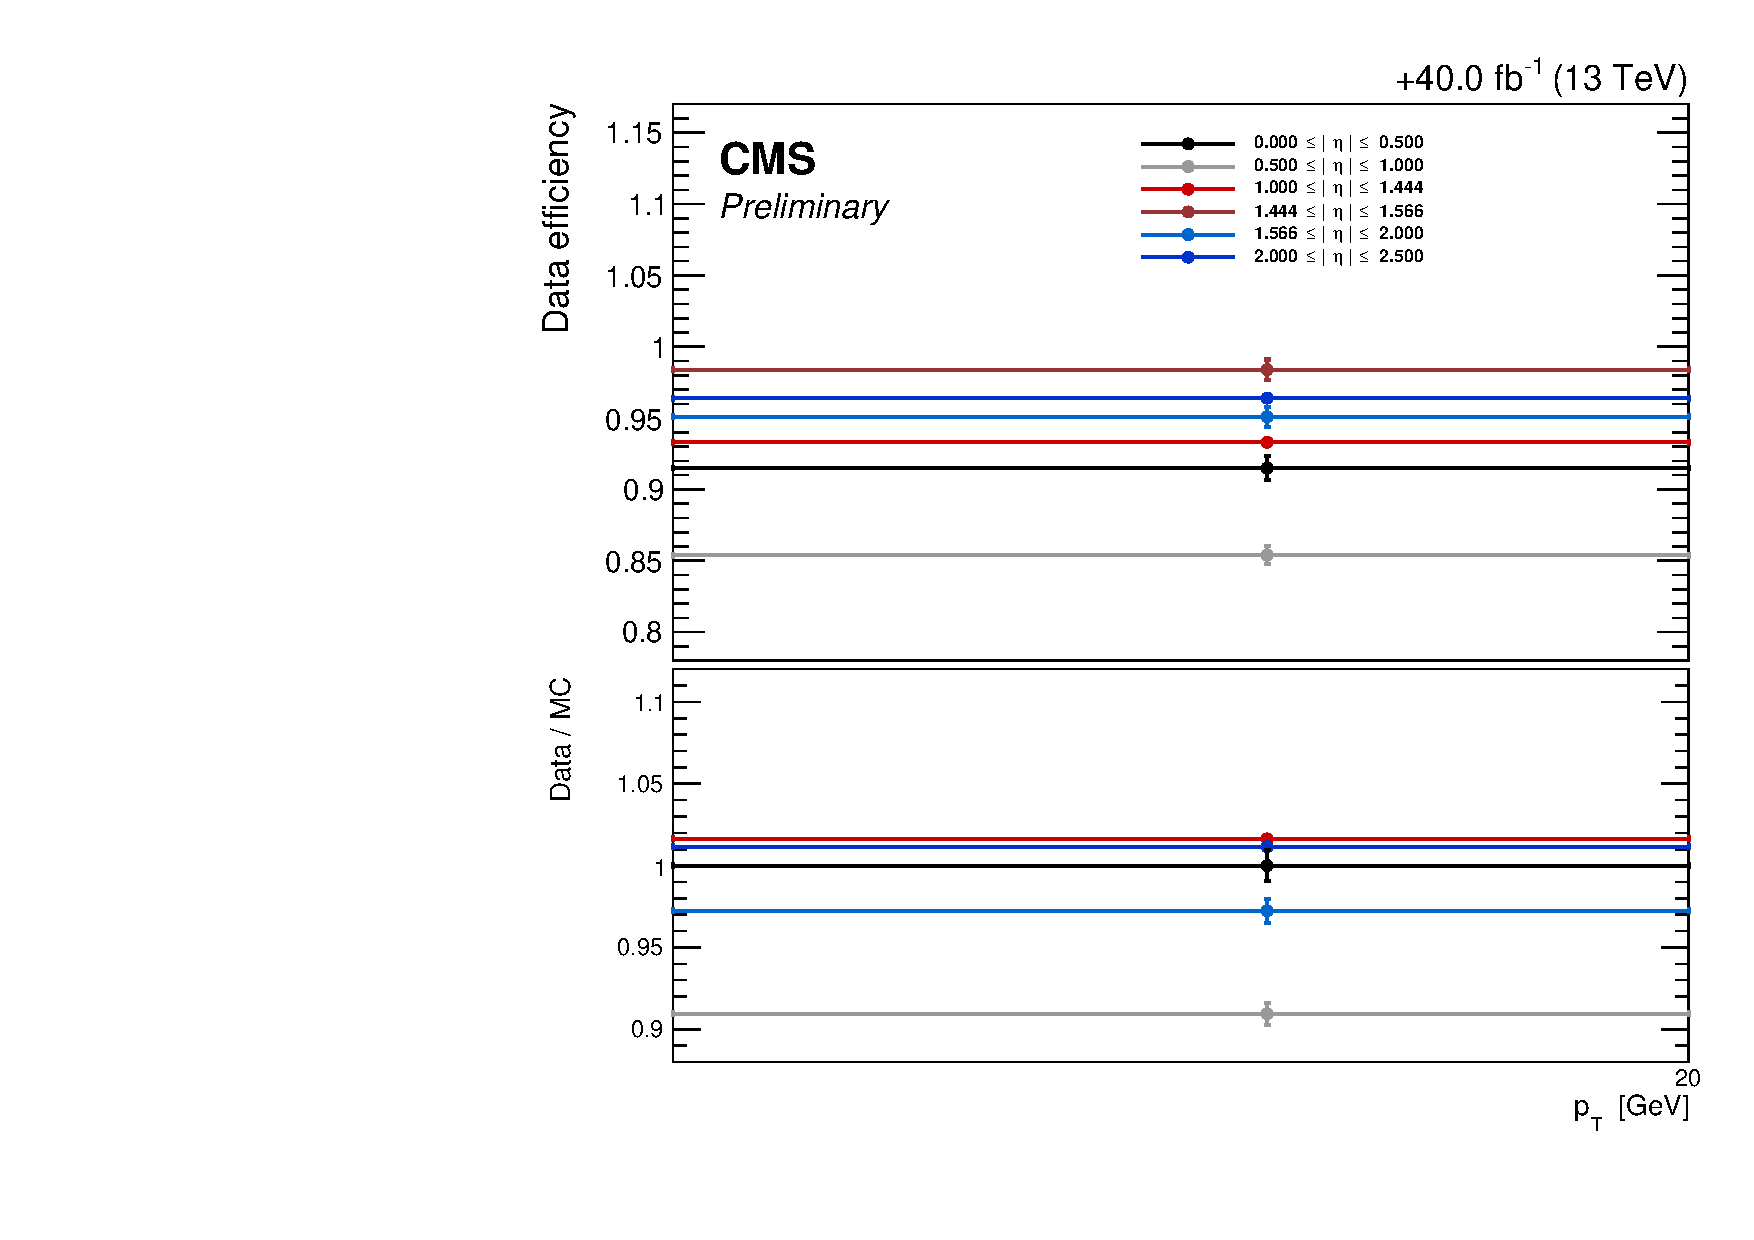
\includegraphics[width=0.4\textwidth]{Figures/Electrons/ErecoPt_lowPt}
%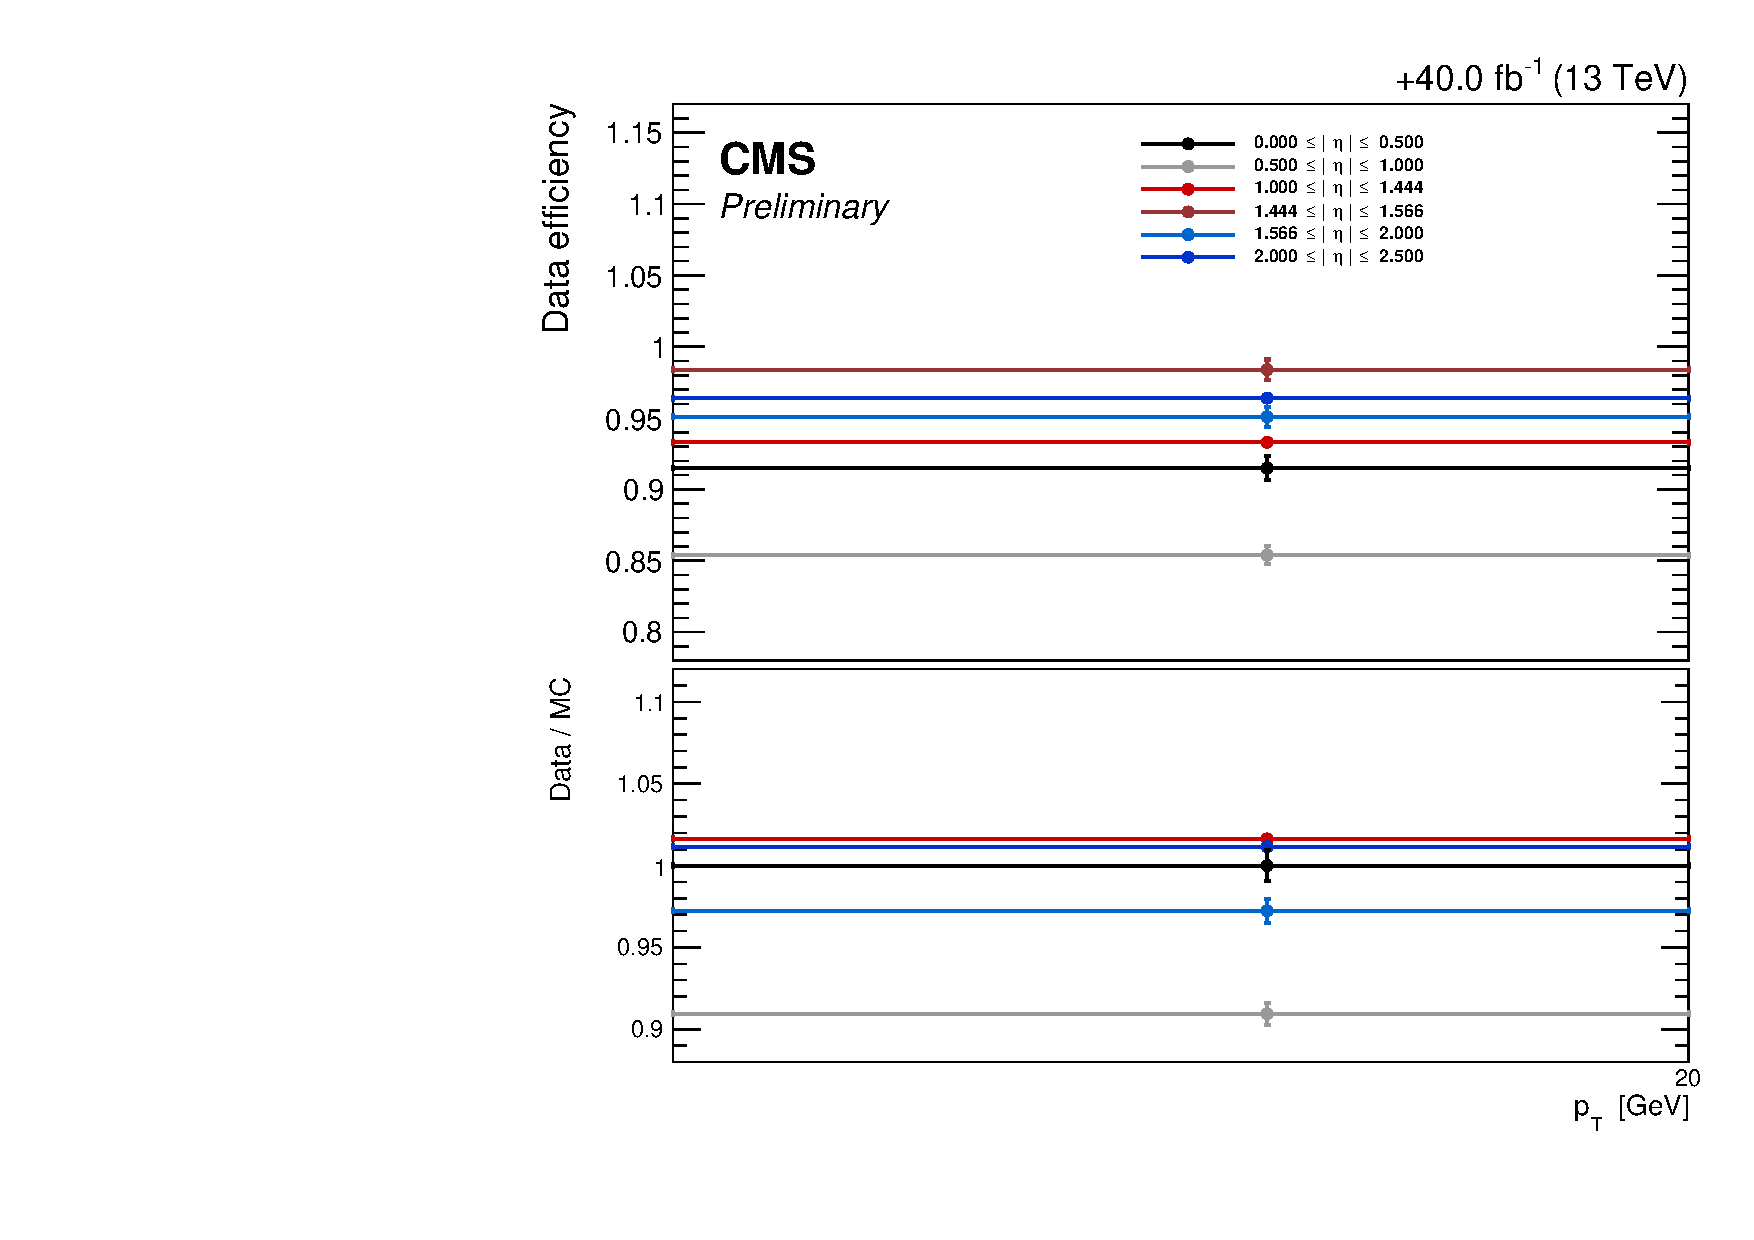
\includegraphics[width=0.4\textwidth]{Figures/Electrons/ErecoEta_lowPt}
\end{center}
\caption{Reconstruction efficiencies of electron in data versus $p_T$ (left), $\eta$ (right) for electrons having $\pt > 20 \GeV$ (top) and $\pt < 20 \GeV$ (bottom) with corresponding data/MC scale factors as provided by the EGM POG.}
\label{fig:ele_rec_scale_factors}
\end{figure}


